\documentclass[main.tex]{subfiles}

\begin{document}    
\chapter{Fundamentals}
This chapter is dedicated to covering the different topics required for understanding the analytical and numerical aspects of our parton shower formalism. Most of the results given in this chapter will be simply quoted from known texts, and formal derivations will generally not be recreated. The topics to be covered is quantum chromodynamics, heavy-ion collisions, and kinematics of parton branchings. The first of these is a pure theoretical framework for the strong nuclear force, while the second will serve as a segway from this theory into the world of heavy-ion collisions. The third topic is a bit more specific for the principles required for discussing parton showers, and implementing them into Monte-Carlo programs.

\section{Quantum Chromodynamics}\label{sec: QCD}
Quantum chromodynamics (QCD) is the theory describing the strong interaction, on of the four fundamental forces in nature. It is a quantum field theory and is a part of the famous standard model.

Historically there were several problems QCD tried to address. Among them where the ratio of the hadronic cross section to the muon-pair cross section produced by \(e^+e^-\)  interactions, \(R = \frac{\sigma(e^+e^-\rightarrow\text{hadrons})}{\sigma(e^+e^- \rightarrow \mu^+\mu^-)}\), which was off by a factor of three in the calculation. Another issue that was yet to be addressed was the existence of the \(\Omega^-\) particle, which consists of three strange quarks giving it a symmetrical wave function in violation of the Pauli principle. It was also unclear at the time why members of the triplet representations of the SU(3) group with fractional charges (\(\frac{2}{3}\) and \(-\frac{1}{3}\)) were unobserved in experiments \cite{CERN_courier_History_of_QCD}. 

The addition of the color degree of freedom resolved all of these challenges. By allowing for three different colors, the \(R\) ratio gained a factor three. The \(\Omega^-\) could now have an anti-symmetric wave function as there were now another quantum number with three different values. The elusive fractionally charged hadrons were also accounted for by assuming that hadrons can only form as colorless states, this will be further explored in the section on confinement. As the name implies, quantum chromodynamics is the theory of color, and it is not without reason.

Beginning this chapter we will explore the basics of QCD, including how the concept of color manifests, how casimirs (color factors) originate from the generators of the SU(3) symmetry, and then a short overview of the Lagrangian and the first-order Feynman diagrams in QCD. Following that the concept of confinement will be explored. Finally the concept of the running coupling, or asymptotic freedom, which defines how the strength of the strong interactions changes with scale and distance, will be introduced.

\subsection{The basics of QCD}
\subsubsection*{Group theory}
Formally quantum chromodynamics is a non-abelian gauge theory described by the SU(3) symmetry, which is a Lie group. The generators of the group are defined from the traceless hermitian Gell-Mann matrices \(\lambda_a\) which are given in \autoref{eqn: gell_mann_matrices}. 
\begin{align}\label{eqn: gell_mann_matrices}
    \begin{split}
    \lambda_1 = \mqty(0&1&0\\1&0&0\\0&0&0) \quad, \quad \lambda_2 &= \mqty(0&-i&0\\i&0&0\\0&0&0) \quad, \quad \lambda_3 = \mqty(1&0&0\\0&-1&0\\0&0&0) \\
    \lambda_4 = \mqty(0&0&1\\0&0&0\\1&0&0) \quad, \quad \lambda_5 &= \mqty(0&0&-i\\0&0&0\\i&0&0)\\
    \lambda_6 = \mqty(0&0&0\\0&0&1\\0&1&0) \quad ,\quad \lambda_7 &= \mqty(0&0&0\\0&0&-i\\0&i&0) \quad, \quad \lambda_8 = \frac{1}{\sqrt{3}} \mqty(1&0&0\\0&1&0\\0&0&-2) 
    \end{split}
\end{align}
The generators \(T^a\) of QCD satisfy \(\left[T^a, T^b\right] = i \, f^{abc}\, T^c\), which is the Lie Algebra of the SU(3) group. Here \(f^{abc}\) is called the \emph{structure constants}, and physicists generally choose to normalize them as \(\Sigma_{c,d}f^{acd}\, f^{bcd} = N \delta^{ab}\). The normalization of the generators follows naturally \cite[p.485]{schwartz2014quantum}. 
\begin{equation}\label{eqn: color_operators}
    T^a = \frac{1}{2}\, \lambda_a \quad, \qquad (a=1,2,\cdots, 8)
\end{equation}
The generators are also called \emph{color operators}, and they act on the color wavefunctions \(\chi^c\). For a single quark the wavefunction is written as a product of the space/spin part \(\psi\), and the color \(\chi^c\). The three color wavefunctions are denoted \(\chi^c = r,b,g\) and are represented by the color spinors, 
\begin{equation}\label{eqn: color_spinors}
    r = \mqty(1\\0\\0) \quad, \quad g = \mqty(0\\1\\0) \quad, \quad b = \mqty(0\\0\\1)
\end{equation}
When examining the color operators it can be noted that the only two of them commute, \(T^3\) and \(T^8\). The color states \(\chi^c =a,b,c\) are therefore eigenstates of both these operators, and do not change the color state they are acting on. This naturally means that the remainder of the color operators are non-diagonal, which means that the interaction can annihilate quarks of one color, and create quarks of a different color. This is an important feature which is unique to QCD, and by conservation of color the gluons must also have non-zero color charges, and therefore be able to self-interact.

The color operators will inevitably allow us to introduce eight real gauge fields \(\mathbf{A}_\mu = A_\mu^a \lambda_a\), which corresponds to the octet of vector gauge bosons - the eight gluon fields.

The generators as presented here is the fundamental representation of the SU(3) group, meaning that it is the smallest non-trivial representation of the algebra. It is the most important representation, along with the adjoint representation described by \((T^a_{\text{adj}})^{bc}=-if^{abc}\). It is important to have a basis-independent way of characterizing the different representations, and this is done by \emph{Casimirs}. The quadratic casimir of a representation \(R\) is defined as \(T_R^aT_R^a = C_2(R) \mathbf{1}\). For evaluating the quadratic casimir, it will be useful define an inner product for the generators as \(\text{tr}\left[T_R^aT_R^b\right]=T(R)\delta^{ab}\). The number \(C(R)\) is then known as the index of the representation. For a given SU(N) group the index \(T_R\) and quadratic casimir \(C_R\) of a given representation \(R\) is given by \autoref{eqn: casimirs} \cite[p.484-489]{schwartz2014quantum}. These quantities appear in almost every calculation in QCD. 
\begin{align}\label{eqn: casimirs}
    T_A = C_A = N \quad, \qquad T_F = \frac{1}{2}  \quad, \qquad C_F = \frac{N^2-1}{2N}
\end{align}

\subsubsection*{The QCD Lagrangian}
Since QCD is a quantum field theory it has a \emph{Lagrangian} which describes the free and interacting parts of the particle fields. We will not do any formal derivation, but will be motivating the relevant results given by standard textbooks. The Yang-Mills is given by \autoref{eqn: yangmills_lagrangian_mandlshaw_11.35}\cite{Peskin:1995ev},
\begin{align}\label{eqn: yangmills_lagrangian_mandlshaw_11.35}
    \begin{split}
    \mathcal{L}_{\textit{QCD}} &= \bar \Psi^f(x) \left[ i \slashed D -m_f\right] \Psi^f(x) - \frac{1}{4} G_{i\mu\nu}(x)G_{i}^{\mu\nu}(x)
    \end{split}
\end{align}
Here the gluon term and covariant derivative is defined as, 
\begin{align}
    G_i^{\mu\nu}(x) &= \partial^\nu A_i^\mu(x) - \partial^\mu A_i^\nu(x) + g_S f_{ijk}A_j^\mu(x)A_k^\nu(x) \\
    D^\mu \Psi^f(x) &= \left[\partial^\mu + ig_S \lambda_j A_j^\mu(x)/2 \right]\Psi^f(x)
\end{align}
The gluon term corresponds to free gluons, with an additional interaction term for achieving gauge-invariance. The covariant derivative then ensures invariance under local phase transformations\cite{mandl2010quantum}.
The Lagrangian of \autoref{eqn: yangmills_lagrangian_mandlshaw_11.35} is therefore gauge invariant. It is therefore not suitable for quantization as the path integral formulation gives no methods for selecting among equivalent solutions, which we have due to gauge invariance. This is resolved by the Faadeev-Popov method which fixes our choice of gauge by adding a gauge fixing term to the Lagrangian. We will now explore two different choices of gauge, the \emph{Feynman gauge}, and the \emph{lightcone gauge}.

\subsubsection*{Feynman gauge}
The first type of gauge we will examine is the covariant \(R_\xi\) gauges introduced by the gauge fixing,
\begin{equation}\label{eqn: gauge_fixing_Rxi}
    \mathcal{L}_{\text{gauge-fix}} = -\frac{1}{2\lambda} \left(\partial_\mu A_i^\mu(x)\right)^2 
\end{equation}
These gauges preserve Lorentz invariance and give simpler calculations than non-covariant gauges. We will be working with the Feynman gauge which is obtained by setting \(\lambda =1\) in the gauge fixing, which is typical for most field theory calculations.

The consequence of choosing covariant gauges is that we are no longer guaranteed that only physical transverse modes of \(A_\mu^a\) propagate, and we get additional kinetic terms which are ghost-like, giving us ghost fields \(\eta_i(x)\). These fields correspond to unphysical spin-0 fermions which can only appear as virtual particles in loop corrections  \cite{schwartz2014quantum, mandl2010quantum}. Introducing the gauge-fixing term of the Feynman gauge and resulting ghost fields to our Lagrangian it takes the form \autoref{eqn: QCD_Lagrangian_feynman_gaugefixghost},
\begin{align}\label{eqn: QCD_Lagrangian_feynman_gaugefixghost}
    \begin{split}
    \mathcal{L}_{\textit{QCD}} &= \bar \Psi^f(x) \left[ i \slashed D -m_f\right] \Psi^f(x) - \frac{1}{4} G_{i\mu\nu}(x)G_{i}^{\mu\nu}(x) \\
    &\quad - \frac{1}{2\lambda} \left( \partial_\mu A_i^\mu(x)\right)^2 + \partial_\nu \eta_i(x) \left[\partial^\nu \tilde \eta_i(x)+g_S f_{ijk} \tilde\eta_j(x) A_k^\mu(x)\right]
    \end{split}
\end{align}
The gluon propagator in the Feynman gauge is given as,
\begin{equation}\label{eqn: gluon_propagator_feynman}
    i \Pi_{\text{feynman}}^{\mu\nu ab} = \frac{-i g^{\mu\nu}}{p^2+i\epsilon} \delta^{ab}
\end{equation}
We will be using this propagator when doing calculations. 

\subsubsection*{The lightcone gauge}
We will now turn to the lightcone gauge which is a type of axial gauge. Axial gauges violate Lorentz invariance, and makes it such that ghosts decouple from the physical particles, and can be ignored altogether. The gauge fixing of axial gauges is given by, 
\begin{equation}\label{eqn: gauge_fixing_axial}
    \mathcal{L}_{\text{gauge-fix}} = -\frac{1}{2\lambda} \left(n_\mu A_i^\mu(x)\right)^2 
\end{equation}
where \(n_\mu\) is some vector. The lightcone gauge is then defined from \(n^2 = 0\) and \(\lambda = 0\), meaning that \(n_\mu\) is light-like. The gluon propagator in the lightcone gauge is given as,
\begin{equation}\label{eqn: gluon_propagator_lightcone}
    i \Pi_{\text{lightcone}}^{\mu\nu ab} = \frac{i}{p^2+i\epsilon} \left[-g^{\mu\nu}+ \frac{r^\mu p^\nu+p^\mu r^\nu}{rp} \right]\delta^{ab}
\end{equation}
There are only two physical polarizations in the lightcone gauge, those transverse to the \(r-p\) plane. The numerator of the propagator is the poalrization sum of transversemodes in a given basis, since there is only two polarizations being propagated, we don't need ghosts to eliminate unphysical polarizations.  

Axial gauges are not really useful unless there is some natural direction to choose. It is therefore very applicable in heavy-ion collisions, as we generally have an initial parton travelling in some direction which an define the vector \(n_\mu\). 


\subsubsection*{Feynman diagrams}
Since we are generally conserned with interactions it is possible to expand the terms of of our Lagrangian in Feynman gauge, \autoref{eqn: QCD_Lagrangian_feynman_gaugefixghost}, and isolate the interaction parts of the Lagrangian for quarks, gluons, and ghosts, we then obtain,
\begin{align}
    \mathcal{L}_{\mathcal{I}\textit{quark}} &= - \frac{1}{2} g_s \bar \Psi^f(x) \gamma_\mu \lambda_j \Psi^f(x) A_j^\mu (x) \label{eqn: QCD_Lpart_quark}  \\
    \begin{split}
    \mathcal{L}_{\mathcal{I}\textit{gluon}} &= g_s f_{ijk} A_{i\mu}(x)A_{j\nu}(x) \partial^\mu A_k^\nu(x) \\
    &\quad - \frac{1}{4} g_s^2 f_{ijk} f_{ilm} A_j^\mu(x) A_k^\nu(x) A_{l\mu}(x) A_{m\nu}(x) \label{eqn: QCD_Lpart_gluon} \end{split} \\
    \mathcal{L}_{\mathcal{I}\textit{ghost}} &= g_s f_{ijk} (\partial_\mu \eta_i(x)) \Tilde{\eta}_j(x) A_k^\mu(x) \label{eqn: QCD_Lpart_ghost} 
\end{align}
From these interaction-terms the famous Feynman diagrams can be obtained. \autoref{eqn: QCD_Lpart_quark} gives us a single three-point vertex which gives rise to two diagrams (depending on how the contractions is done), with two quarks and one gluon in each. The diagram is pictured in \autoref{fig: feynman_quark_interactions}. The gluonic contribution to the lagrangian gives us two different terms containing exclusively gluon fields, demonstrating the gluon self-interaction we expected from the color operators. The result is the three-gluon vertex and the four-gluon vertex as pictured in \autoref{fig: feynman_gluon_interactions}. The ghost term also gives rise to a Feynman diagram, but it can only occur in virtual loops.
%Full lagrangian:
%\begin{align}\label{eqn: QCD_Lagrangian_Full} \begin{split} \mathcal{L}_{\textit{full}} &= \bar \Psi^f(x) \left[ i \slashed \partial -m_f\right] \Psi^f(x) - \frac{1}{2} g_s \bar \Psi^f(x) \gamma_\mu \lambda_j \Psi^f(x) A_j^\mu (x) \\ &- \frac{1}{4} F_{i\mu\nu}(x) F_i^{\mu\nu}(x) - \frac{1}{2} \left( \partial_\mu A_i^\mu(x)\right)^2  \\ &+ g_s f_{ijk} A_{i\mu}(x)A_{j\nu}(x) \partial^\mu A_k^\nu(x) - \frac{1}{4} g_s^2 f_{ijk} f_{ilm} A_j^\mu(x) A_k^\nu(x) A_{l\mu}(x) A_{m\nu}(x) \\ &+ \partial_\mu \eta_i (x) \partial^\mu \Tilde{\eta}_i(x) + g_s f_{ijk} (\partial_\mu \eta_i(x)) \Tilde{\eta}_j(x) A_k^\mu(x) \end{split} \end{align}

\begin{figure}[htb]
    \centering
    \begin{minipage}{.35\textwidth}
    \centering
        \begin{tikzpicture}
            \begin{feynman}
            \vertex (a);
            \vertex [right=of a] (v);
            \vertex [above right=of v] (b);
            \vertex [below right=of v] (c);
            \diagram* {
            (a) -- [gluon, edge label = \(k_1 \) ] (v),
            (v) -- [fermion, edge label' = \(k_2 \) ] (b),
            (v) -- [anti fermion, edge label = \(k_3 \) ] (c),
            };
            \end{feynman}
        \end{tikzpicture}
  \label{fig:test1}
\end{minipage}%
\begin{minipage}{.35\textwidth}
    \centering
        \begin{tikzpicture}
            \begin{feynman}
            \vertex (a);
            \vertex [right=of a] (v);
            \vertex [above right=of v] (b);
            \vertex [below right=of v] (c);
            \diagram* {
            (a) -- [fermion, edge label = \(k_1 \) ] (v),
            (v) -- [fermion, edge label' = \(k_2 \) ] (b),
            (v) -- [gluon, edge label = \(k_3 \) ] (c),
            };
            \end{feynman}
        \end{tikzpicture}
\end{minipage}
\caption{Feynman diagrams of the quark-gluon interactions arising from the QCD lagrangian.}
\label{fig: feynman_quark_interactions}
\end{figure}
\begin{figure}[htb]
    \centering
    \begin{minipage}{.35\textwidth}
    \centering
      \begin{tikzpicture}
            \begin{feynman}
            \vertex (a);
            \vertex [below=of a] (v);
            \vertex [below right=of v] (b);
            \vertex [below left=of v] (c);
            \diagram* {
            (a) -- [gluon, edge label = \(k_1 \) ] (v),
            (b) -- [gluon, edge label' = \(k_2 \) ] (v),
            (c) -- [gluon, edge label = \(k_3 \) ] (v),
            };
            \end{feynman}
        \end{tikzpicture}
\end{minipage}%
\begin{minipage}{.35\textwidth}
    \centering
        \begin{tikzpicture}
            \begin{feynman}
            \vertex (a);
            \vertex [below right=of a] (v);
            \vertex [above right=of v] (b);
            \vertex [below right=of v] (c);
            \vertex [below left=of v] (d);
            \diagram* {
            (a) -- [gluon, edge label' = \(k_1 \) ] (v),
            (b) -- [gluon, edge label = \(k_4 \) ] (v),
            (c) -- [gluon, edge label' = \(k_3 \) ] (v),
            (d) -- [gluon, edge label = \(k_2 \) ] (v),
            };
            \end{feynman}
        \end{tikzpicture}
\end{minipage}
\caption{Feynman diagrams of the gluon self-interactions arising from the QCD lagrangian.}
\label{fig: feynman_gluon_interactions}
\end{figure}

These are all of the first-order interactions of QCD. There are naturally higher-order diagrams and loop-corrections which may pose challenges when dealing with calculations, but for our purposes the first-order terms are sufficient. 

\subsection{Confinement}
Confinement is the phenomenon that particles with color charge can not exist as isolated particles under normal conditions of temperature and pressure. While it is not fully understood how it emerges from the Lagrangian of QCD, it remains as an experimental fact - quarks and gluons are forced to be bound into color-neutral states called hadrons. The simplest example is mesons which consists of a quark and an anti-quark of the same flavor, and is obviously color-neutral. 

The familiar Coulomb potential of QED is attractive for opposite charges, and repulsive for similar charges. It would therefore be interesting to observe how the QCD potential would be for quark anti-quark pairs, of similar and different color charge. For large separations the potential increases linearly \(V(r) \sim k\, r\). For small separations the a potential similar to the Coulomb will dominate as calculated in \cite[p.512-513]{schwartz2014quantum}. Combining these the total potential \(V_{\text{QCD}}\) takes the form,
\begin{align}\label{eqn: QCD_potential}
    \begin{split}
    V_{\text{QCD}}(r) &= k\,r - \frac{4}{3} \frac{g_s^2}{4\pi r} \quad, \qquad \text{color singlet} \\
    V_{\text{QCD}}(r) &= k\,r + \frac{1}{6} \frac{g_s^2}{4\pi r} \quad, \qquad \text{color octet}
    \end{split}
\end{align}
The color singlet represents the potential for \(q \bar q\)-pairs of the same color charge, and is the only one that is attractive for small separations. This is consistent with our expectations that quarks can form color neutral mesons. The color octet which is all combinations of \(q \bar q\)-pairs of different color charge is however repulsive for all \(r\), and mesons with a net color charge does not form. 

An interesting part of confinement should now become apparent from examining the potential between a \(q \bar q\)-pair of similar color charge. If we were try to forcefully separate the quarks, the potential between them would eventually become great enough for it to be energetically favorable to form a new \(q \bar q\)-pair which forms with the existing pair, giving us two mesons. This property is illustrated by the famous rubber band analogy in \autoref{fig: QCD_rubberband}. 
\begin{figure}[htb]
    \centering
    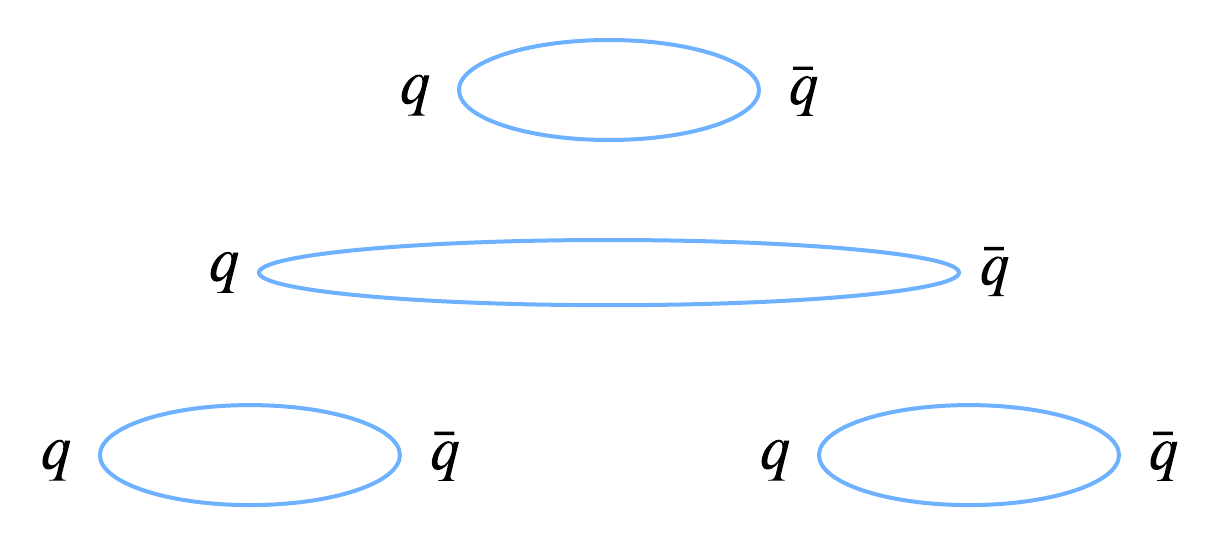
\includegraphics[width=9cm]{pictures/figures/QCD_potential_rubberband.png}
    \caption{When the potential between a \(q\bar q\)-pair becomes too large, it is energetically favorable to create a new \(q\bar q\)-pair. This can be visualized like pulling a rubber band that, instead of breaking, spontaneously turns into two new rubber bands.}
    \label{fig: QCD_rubberband}
\end{figure}

\subsection{The running coupling}
Field theories such as QED and QCD, have a coupling constant which describes the strength of a given interaction, relative to the free fields. For QED this is known from the fine-structure constant \(\alpha \approx \frac{1}{137}\), which is proportional to the squared electric charge \(e^2\), which we intuitively can understand as how strongly an electrically charged particle interactions with an electrical field. The same goes for QCD, where the coupling constant \(g_s\) only appears in the interaction-parts of the Lagrangian. Higher order interactions scale with orders of the coupling constant, as is apparent in the interaction-part of the gluon Lagrangian \autoref{eqn: QCD_Lpart_gluon} where the three-gluon vertex is scaled by \(g_s\), and the four-gluon vertex is scaled by \(g_s^2\). 

The QCD Lagrangian given by \autoref{eqn: yangmills_lagrangian_mandlshaw_11.35} contains the bare coupling constant \(g_s\). This is only valid for tree-level in perturbation theory, and needs to be corrected by the method of \emph{renormalization} to account for divergences appearing from higher order loop corrections. Renormalization will allow us to replace the bare coupling constant with a renormalized coupling constant \(g_r(\mu)\), where \(\mu\) is an scale dependence which is a consequence of the renormalization procedure. It is customary to define this new coupling in analogy to the fine-structure constant such that \(\alpha_s(\mu)=\frac{g_r^2}{4\pi}\), this new coupling is given from 
\begin{equation}\label{eqn: coupling_QCD_running}
    \alpha_s(\mu) = \frac{2\pi}{\beta_0 \ln(\mu^2/\Lambda_{\text{QCD}}^2)}
\end{equation}
In this new coupling constant, the \emph{\(\beta\)-function} encodes the dependence of the coupling changes with scale, without having an explicit \(\mu\) dependence. The \(\beta\)-function is therefore responsible for the running of the coupling constant. \(\Lambda_{\text{QCD}}\) is the scale at which the coupling constant becomes infinite, also called the Landau pole, and for QCD this scale is typically \(\Lambda_{\text{QCD}} \sim 0.2 \text{GeV}\). 

\krs{Insert graph?}

The importance of the running coupling in QCD is that \(\alpha_s(\mu)\rightarrow 0\) as \(\mu\rightarrow \infty\). This is known as \textit{asymptotic freedom}. For processes with a large momentum transfer \(Q>>\Lambda_{\text{QCD}}\), such as high energy jets, the process can be described by perturbation theory. The uniqueness of the running coupling in QCD is that the \(\beta\)-function is negative, which gives rise to confinement \cite{Caucal:2020zcz}.

\subsection{Quark-Gluon plasma}
In our discussion on confinement we made an explicit statement that particles with color charge can not exist as isolated particles under "normal conditions of temperature and pressure". This naturally sparks the question of what happens under extreme conditions of high temperature and pressure.

At increasing temperature and/or increasing baryon density a phase transition occurs such that hadrons no longer exist. The resulting matter consisting of free quarks and gluons is commonly called the \emph{quark-gluon plasma} (QGP). While it is commonly called a plasma it is not always clear weather it should be interpreted as a weakly interacting gas, or a strongly correlated system such as a fluid. 
The properties of the quark-gluon plasma is best illustrated using a phase diagram such as the one given in \autoref{fig: QCD_phasediagram}. 
\begin{figure}[htb]
    \centering
    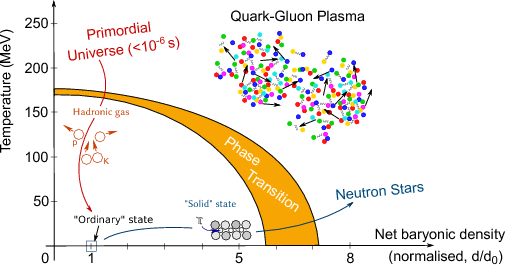
\includegraphics[width=9cm]{pictures/figures/QGP_phasediagram.png}
    \caption{Typical phase diagram for QCD matter, ranging from regular nuclear matter to quark-gluon Plasma. Boundaries are not necessarily exact. Figure from \cite{QCD_phasediagram_MaireAntonin}.}
    \label{fig: QCD_phasediagram}
\end{figure}

There are several points of interest in this phase diagram. The most obvious feature is the phase transition between the hadron gas and the quark-gluon plasma, which is defining feature of QGP and he violation of confinement, called \emph{deconfinement}, under extreme conditions. There is however another transistion which may occur which is the \emph{chiral phase transition}. In short QCD has a unique feature that chiral symmetry is broken, meaning that the theory acts differently on left- and right-handed fields. This is however restored for high pressure and/or temperature. Currently it seems like the two phase transitions occur simultaneously \cite{florkowski2010phenomenology}.

Studying the QGP is difficult as it is very short lived and difficult to probe or measure directly. The main method of identifying QGP is to observe how highly energetic partons interact with the plasma in the immediate aftermath of heavy-ion collisions (\(Au+Au\)), at colliders such at RHIC and LHC. These high energy particles, called \emph{jets}, eventually lead to collimated groups of hadrons, or \emph{parton showers}, which are observed in our detectors.

\section{Properties of relativistic heavy-ion collisions}
A jet is a narrow cone of particles, which are produced by the hadronization of a quark or gluon in the aftermath of relativistic heavy-ion collision. Jets is the currently the only way of probing the QGP. We will now explore the evolution of heavy-ion collisions, typically \(P_b-P_b\) collisions,  from the impact all the way to the detector. Properties of the jets and its observables will be accounted for, alongside the basic terminology used for parton branching. Then we will see jets interact with the medium and gives rise to broadening.

\subsection{Evolution of relativistic heavy-ion collisions}
The different phases and time evolution relativistic heavy-ion collisions is given from \autoref{fig: evolution-heavy-ion-collisions}. The units of the diagram is \(fm/c=3.3\cdot 10^{-24}s\). The first stage of the evolution is the pre-equilibrium dynamics where partons (mostly gluons) are quickly freed by the collision, and then start to approach thermal equilibrium. This gives us the initial energy density around \(1fm/c\) which is the basis for the quark-gluon plasma phase which evolves until around \(10fm/c\). When the baryon density and temperature becomes too small for deconfinement, hadrons are formed, a process called \emph{hadronization}. The hadron gas is treated using relativistic hydrodynamics, until it cools enough for the \textit{freeze-out}, which finally leaves us with the free hadrons which we finally observe in our detector. 
\begin{figure}[htb]
    \centering
    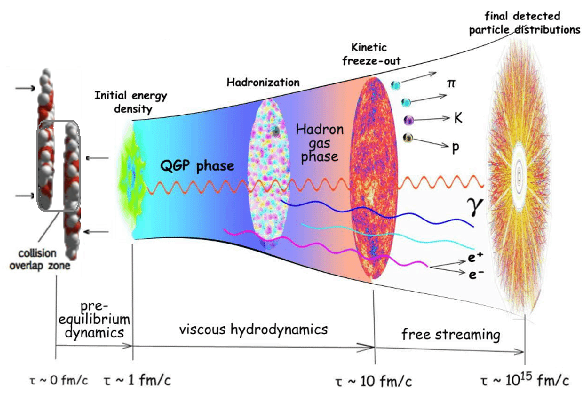
\includegraphics[width=12cm]{pictures/figures/evolution-of-relativistic-heavy-ion-collisions.png}
    \caption{Illustration of the dynamical evolution of relativistic heavy-ion collisions. Evolution starts at the initial collision and continues until the hadronized particles reach the detector. The bottom axis gives the time scale of the evolution, and the dynamics governing the system. Figure from \cite{QCD_figures/Scharenberg}, colors are inverted.}
    \label{fig: evolution-heavy-ion-collisions}
\end{figure}

For this thesis we are interested in the high-energy partons at the very start of the QGP phase, as these will lead to jets and eventually the parton showers we observe in the detector, by the process of \emph{parton branching}.

Parton branching is simply the process of an energetic parton splitting into two new partons. This can happen via all of the basic QCD vertices and allows for the number of partons in a jet to increase, which leads to hadronization and eventually the parton showers we observe in detectors. When addressing parton branching we will generally mean \emph{collinear branching}, where the newly created parton travels in the same direction as the branching parton. This implies naturally that the opening angle of the branching is very small. Somewhat analogous to parton branching we have \emph{gluon radiation}. In principle it is the same thing but when speaking of gluon radiation we generally mean that interactions with the medium has caused an energetic parton to emit a \emph{soft gluon}, often referenced as induced gluon radiation. These soft gluons carry very little momentum, and is typically emitted at larger angles. The softer the emission, the larger the emission angle \cite{medium_induced_gluon_branching}.

Jets and parton branching will be explored both for vacuum and medium evolutions, where the latter gives us the phenomena of \emph{broadening} and \emph{quenching}, due to interactions with the quark-gluon plasma.

\krs{add double log / leading log?}


\subsection{Angular ordering}
The parton showers presented here will be angular ordered, meaning that any subsequent emission angles are smaller than the previous angle. For simple parton branchings angular ordering can be obtained by considering the spatial separation of the daughter-partons of the branching.
\begin{figure}[htb]
    \centering
        \begin{tikzpicture}
            \begin{feynman}
            \vertex (a);
            \vertex [right=of a] (a1);
            \vertex [right=of a1] (v);
            \vertex [above right=of v] (v1);
            \vertex [above right=of v1] (v2);
            \vertex [above right=of v2] (v3);
            \vertex [above right=of v3] (f1);
            \vertex [right=of v2] (v5);
            \vertex [right=of v5] (f3);
            \vertex [below right=of v] (v10);
            \vertex [below right=of v10] (f2);
            \diagram* {
            (a) -- [gluon, edge label = \(a\)] (v),
            (v) -- [gluon, edge label = \(c\)] (f1),
            (f2) -- [gluon, edge label = \(b\)] (v),
            (f3) -- [gluon, edge label = \(d\)] (v2),
            (v5) -- [scalar, quarter right,opacity = 0.5, edge label = \(\theta \) ] (v3),
            (v10) -- [scalar, quarter right,opacity = 0.5, edge label = \(\theta_0 \) ] (v1),
            (f3) -- [opacity = 0] (f1),
            (v2) -- [ghost, opacity = 0.5, edge label = \(r_\perp\)] (f2),
            };
            \end{feynman}
        \end{tikzpicture}
\caption{Illustration of the opening angles for successive parton branchings.}
\label{fig: angular_ordering}
\end{figure}

Looking at \autoref{fig: angular_ordering}, we have noted the opening angle of the initial branching as \(\theta_0\), and the successive branching as \(\theta\). If the secondary branching parton has a wavelength \(\lambda \sim \frac{1}{k_\perp} \sim \frac{1}{\omega \theta}\), and formation time \(t_f\sim \omega/k_\perp^2\), then the formation time can be written, 
\begin{equation}
    t_f \sim \frac{\omega}{k_\perp^2} = \frac{1}{\omega \theta^2}
\end{equation}
The spatial separation of the partons from the initial branching can be given from the same formation time as \(r_\perp \sim \theta_0\, t_f = \frac{\theta_0}{\omega \theta^2}\). Imposing the criteria that the wavelength \(\lambda\) of the branched parton \(d\) must be smaller than the separation distance \(r_\perp\)
\begin{align}\label{eqn: angular_ordering}
    \lambda &< r_\perp \nonumber \\
    \frac{1}{\omega \theta} &< \frac{\theta_0}{\omega \theta^2} \nonumber \\
    \theta &< \theta_0
\end{align}
The criteria \(\lambda < r_\perp\) leads us therefore to angular ordering. The reasoning for us to be able to impose this criteria originates from our desire to have \emph{resolvable} branchings. This means that the branched parton \(d\) should be able to probe weather it branched from \(c\), or from \(b\). This is also called \emph{coherent branching}. If the wavelength of \(d\) is too large, then it will not be able to distinguish, or resolve, \(b\) and \(c\) as individual partons, and it would instead branch from the sum of the color charges, which is equivalent to branching from \(a\) \cite{Dokshitzer:1991wu}. When we are constructing our Monte-Carlo program we will be using the angle \(\theta\) as our ordering variable, meaning that we start from a large value of \(\theta\) and branch our way down to smaller angles. Angular ordering follows therefore naturally from the choice of variable.

Coherent branchings also imply that color charge is conserved along the parton shower for the same reasons - if the branching is resolvable each successive branching will conserve the net color charge. In medium cascades it is however expected that color is not necessarily conserved along the shower. This is due to the large amount and frequency of soft gluon emissions, which results in incoherent branchings, and the newly emitted gluon will probe the net color charge \cite{medium_induced_gluon_branching}.


\subsection{Broadening}
Broadening takes place during the QGP phase of heavy-ion collisions. The concept is quite simply gluons exchanging transverse momentum with the medium, resulting in a transverse momentum distribution is broader than the initial one. This happens via multiple collisions between the parton and the medium constituents, resulting in induced radiation, primarily soft gluons, with a formation time of \(t_f\sim \omega/k_\perp^2\)\lit{Sometimes given as \(t_f\sim 2\,\omega/k_\perp^2\).}. During this time-scale the gluon can experience multiple kicks which may increase its transverse momentum by a factor \(k_\perp^2 \sim \hat q \,t_f\), where \(\hat q\) is a diffusion coefficient, called the \emph{jet-quenching parameter}. If these kicks from the medium is the only source of transverse momentum, the typical time for emission called the branching time is given by, 
\begin{equation}\label{eqn: branching_time}
    \tau_{br} = \sqrt{\frac{\omega}{\hat q}}
\end{equation}
The dependence on \(\omega\) comes from the simple fact that higher energy partons require more kicks to be put on-shell\textcolor{red}{why does it need to be on shell for branching? - from medium induced gluon branching, Blaizot.}. 
When the collisions are soft, and a large number of collisions is
needed to change the transverse momentum by a significant amount, the diffusion approximation given by \(\hat q\) is valid. The total transverse momentum \(p_\perp\) gained by a high-energy parton traversing a medium of length \(L\) is therefore given by the definition of the diffisuion coefficient to be, 
\begin{equation}\label{eqn: broadening}
    \langle p_\perp^2\rangle = \hat{q}\, L
\end{equation}
The jet-quenching parameter will generally be set to some constant, even tough it is a function of momentum \(\hat q(\vec p^2)\) \cite{Jet_Structure_HeavyIonCollisions}. Quenching is understood as the suppression of high-\(p_T\) hadrons due to energy loss of the most energetic parton of a given jet, commonly known as the leading parton. This energy loss is primarily caused by soft gluon radiation, which is induced by collisions with the medium \cite{medium_induced_gluon_branching}. The concepts of broadening and quenching are closely connected, and both are consequences of medium interactions.

\subsection{Observables}
\krs{Write about transverse momentum?}
This section will present different observables and quantities which will be particularly important for our treatment of parton showers.

The method of grouping different quarks and gluons into the same jet is defined by so called \textit{jet algorithms}. Following the \(k_t-\text{algorithm}\), any quarks or gluons separated by a distance \(\Delta_{ij}^2 = ((y_iy_j)^2+(\phi_i-\phi_j)^2) < R^2\), where R is called the \textit{jet radius}, can be combined into a single jet. The jet radius not an observable for out showers, but it is an important quantity which must be defined for both numerical and analytical purposes \cite{Dasgupta_2015}. 

The most basic jet observable we will encounter is the inclusive jet distribution which contains the information available for all the jets produced by an initial parton. The inclusive jet function \(f_i(x,t)\) is described by the DGLAP evolution equations which will be introduced shortly. Some of the properties of the inclusive jet function are, 
\begin{align}
    \int_0^1 dz\, f_i(x,t) &= \langle N_{i, \text{ jets}}\rangle  \label{eqn: inclusive_function_properties_1}\\
    \int_0^1 dz\, z\,  f_i(x,t) &= 1 \label{eqn: inclusive_function_properties_2}
\end{align}
\autoref{eqn: inclusive_function_properties_1} tells us that the inclusive jet distribution yields the average number of jets. This value is generated dynamically throughout the factorization process, as it depends on the jet radius and scale \(Q\). Since the inclusive distribution gives us the number of jets, it must conserve the momentum as given by \autoref{eqn: inclusive_function_properties_2}. Both of these rules hold only if the inclusive jet functions are written in terms of the initial parton momentum \(Q=p_T\) \cite{Neill_2021}.

When we develop our Monte-Carlo shower program the outcome is a simple list of all final partons which is the jet density \(\frac{dN}{dx}\) and energy density \(x \frac{dN}{dx}\). This is the exact quantities we need to compare with the analytical solution of the jet functions, as should be apparent from the sum rules above.

In contrast to the inclusive jet distributions, the leading jet distribution \(\mathcal{J}(\frac{x}{z},t)\) represents a well-defined object which has lost energy due to out-of-jet emissions. The  sum rules for the leading jets is,
\begin{align}
    \int_0^1 dz\, \mathcal{J}_i(z_{i1},t) &= 1 \label{eqn: leading_function_properties_1}\\
    \int_0^1 dz\, z\,  \mathcal{J}_i(z_{i1},t) &= \langle z_{i1}\rangle  \label{eqn: leading_function_properties_2}
\end{align}
The number of jets is constant in the leading jet distribution, as can be seen from \autoref{eqn: leading_function_properties_1}, and the energy is not conserved as can be seen from \autoref{eqn: leading_function_properties_2}. Since we have an expression for the average energy contained in the leading jet, the average energy loss can be calculated from \(\langle z_{i} \rangle_\text{loss} = 1 -\langle z_{i}\rangle_1 \) \cite{Neill_2021}. 

\section{Kinematics of parton branching}
Taking a step back from the concepts of QCD, this section will discuss the actual kinematics of parton branchings. Beginning with deriving the basic kinematics of vacuum branchings, before we explore the properties and origin of the Alterelli-Parisi splitting functions by considering he matrix-elements of the different QCD vertices. Finally we will take a look at the branching probability by considering the cross-sections of a given process.


\subsection{Kinematic variables}
Rather than obtaining a precise result to some fixed order in perturbation theory, we will rather aim for an approximate result by considering the kinematics of parton branchings, which will valid to all orders, allowing us to introduce a parton shower picture which can be easily implemented into Monte-Carlo programs.

Before doing any calculations the basic kinematic variables must be introduced. Restricting ourselves to the variables which will be used throughout the later sections. We start by considering the branching \(a\rightarrow b,c\) under the assumption that \(p_b^2, p_c^2 << p_a^2 \equiv t\), as illustrated in \autoref{fig: parton_branching1}.
\begin{figure}[htb]
    \centering
    \feynmandiagram [horizontal=a to b] {
    a [blob] -- [gluon, edge label = a] b,
    f1 [particle = b] -- [gluon, edge label = \(\theta_b\)] b  -- [gluon, edge label= \(\theta_c\)] f2 [particle = c],
    f1 -- [opacity=0] f2,};
    \caption{Branching of an outcoming parton \(a\) from some state, into two partons \(b,c\).}
    \label{fig: parton_branching1}
\end{figure}
The opening angle is given as \(\theta = \theta_b+\theta_c\), and the energy carried by the branched partons is given relative to the energy of the parent parton such that if \(E_a =x\), then \(E_b=z\,x,\) and \(E_c=(1-z)\,x\). The relationships between \(z\) and the different energies can therefore be written as,
\begin{equation}\label{eqn: branched_energy_fractions_ellis_5.2}
    z = \frac{E_b}{E_a} = 1- \frac{E_c}{E_a}
\end{equation}
Assuming most of our emissions are \emph{collinear}, the opening angle \(\theta\) is small, and we can use the small angle approximations \(\cos \theta \approx 1- \frac{\theta^2}{2}\) and \(\sin \theta \approx \theta\). Conservation of four-momentum can be used to derive the following relationship between the kinetic variables, assuming the particles are massless, 
\begin{align}
    p_a^2 &= 2 E_b E_c (1-\cos \theta) \nonumber\\ 
    &= 2 \frac{E_b}{E_a} \frac{E_c}{E_a} (1-\cos \theta) E_a^2 \nonumber\\
    &= 2 z (1-z)  (\frac{\theta^2}{2}) E_a^2 \nonumber\\
    &= z (1-z) E_a^2 \theta^2
\end{align}
where the relationships in \autoref{eqn: branched_energy_fractions_ellis_5.2} has been used to introduce \(z(1-z)\). This can be rewritten to give us an expression for the opening angle \(\theta\) in terms of the kinetic variables by using conservation of transverse momentum such that,
\begin{align}\label{eqn: theta_momentum_conv_ellis_5.4}
    z\, E_a \sin \theta_b &= (1-z)\, E_a \sin \theta_c \nonumber \\
    z\, \theta_b &= (1-z)\, \theta_c  \nonumber \\
    \frac{\theta_b}{1-z} &= \frac{\theta_c}{z} = \theta
\end{align}
All of these kinematic variables will be used for deriving the splitting functions for the different QCD vertices. 

\subsection{Altarelli-Parisi splitting functions}\label{sec: derivation_splitting_functions_vacuum}
The Altarelli-Parisi splitting functions \(P_{ba}(z)\) appear when evaluating the matrix elements of the basic QCD vertices. They have a physical interpretation as the probability density of finding a parton \(b\) "inside" of parton \(a\), with a particular momentum fraction \(z\) of the parent parton. This distribution changes with the scale due to its dependence on \(\alpha_S\). The splitting functions are valid as long as the coupling constant is sufficiently small, which for QCD is fulfilled at large scales \cite{AltarelliParisi_original, ellis_stirling_webber_1996}.

Now we will do a re-derivation of the \(P_{\text{gg}}\) splitting function\footnote{The notation for the splitting vertices is such that the first letter gives the parton type with momentum \(z\) after the splitting, and the second letter given the initial parton type. The branching \(a\rightarrow b,c\) is therefore noted as \(ba\).} by identifying the QCD vertex factors of the three-gluon vertex given in \autoref{fig: feynman_gluon_interactions}, and then averaging over incoming and outgoing polarization. The method is outlined in \cite{ellis_stirling_webber_1996}. When taking all the gluon momenta to be incoming, the matrix element \(\mathcal{M}_{n+1}\) will be given by the initial matrix element, \(\mathcal{M}_n\), the gluon propagator \(\Pi^{\mu\nu}\), the vertex factor \(V_{\alpha\beta\gamma}\), and the two final gluon polarization vectors \(\epsilon_b^\beta\epsilon_c^\gamma\), 
\begin{align}
    \mathcal{M}_{n+1} &=  \left( \epsilon_b^\beta \epsilon_c^\gamma  \right) \left(gf_{\alpha\beta\gamma} V_{\alpha\beta\gamma}\right)  \, i \Pi^{\mu\nu ij}\delta_{ij}  |\mathcal{M}_n|
\end{align}
where \(\alpha,\beta,\gamma\) are colour indices. We will start by rewriting the gluon propagator in Feynman gauge \autoref{eqn: gluon_propagator_feynman}, in terms of the gluon polarization states, 
\begin{equation}
    \Pi_{\text{feynman}}^{\mu\nu} = \left(\sum_\lambda \epsilon_\lambda^\mu(p)\, \epsilon_\lambda^{\nu*}(p) \right) \frac{-i}{p^2+i\epsilon}
\end{equation}
One of these gluons will connect to the initial matrix element, while one of them will be connected to our vertex element, 
\begin{align}
    \mathcal{M}_{n+1} &=  \sum_\lambda \left(\epsilon_a^\alpha \epsilon_b^\beta \epsilon_c^\gamma  \right) \left(gf_{\alpha\beta\gamma} V_{\alpha\beta\gamma}\right) \, \frac{-i}{p^2+i\epsilon} \left(\epsilon_\lambda^{\nu*} |\mathcal{M}_{n,\nu}|\right)
\end{align}
Setting \(\frac{1}{t} = \frac{-i}{p^2+i\epsilon} \), squaring the final matrix element, and using the fact that it is proportional to \(1/t\equiv \frac{1}{p^2}\), we obtain the final expression for our vertex element,
\begin{equation}\label{eqn: ggg_matrix_element}
    |\mathcal{M}_{n+1}|^2 \sim \frac{g^2}{t^2} C_A V_{\alpha\beta\gamma}^2  |\mathcal{M}_n|^2
\end{equation}
Continuing lets take a closer look at \(V_{\alpha\beta\gamma}\), which comes from the vertex factor. Since all momenta are incoming, we can use \(p_a +p_b +p_c = 0\), and the condition \(\epsilon_i \cdot p_i = 0\) to rewrite as,
\begin{align}\label{eqn: ggg_vertex_factor_Ellis_5.6}
    V_{\alpha\beta\gamma} &= 
    (\epsilon_a^\alpha \epsilon_b^\beta g_{\alpha\beta})(\epsilon_c^\gamma (p_a-p_b)_\gamma) + 
    (\epsilon_b^\beta \epsilon_c^\gamma g_{\beta\gamma})(\epsilon_a^\alpha (p_b-p_c)_\alpha) + 
    (\epsilon_a^\alpha \epsilon_c^\gamma g_{\gamma\alpha})(\epsilon_b^\beta (p_c-p_a)_\beta) \nonumber \\
    &=
    (\epsilon_a \cdot \epsilon_b)(\epsilon_c^\gamma (-2p_b- p_c)_\gamma) + 
    (\epsilon_b \cdot \epsilon_c)(\epsilon_a^\alpha (2p_b -p_a)_\alpha) + 
    (\epsilon_a \cdot \epsilon_c)(\epsilon_b^\beta (2p_c-p_b)_\beta) \nonumber \\
    &= 
    (\epsilon_a \cdot \epsilon_b)(\epsilon_c \cdot -2p_b) + 
    (\epsilon_b \cdot \epsilon_c)(\epsilon_a \cdot 2p_b) +
    (\epsilon_a \cdot \epsilon_c)(\epsilon_b \cdot 2p_c) \nonumber\\
    &= -2\left(
    (\epsilon_a \cdot \epsilon_b)(\epsilon_c \cdot p_b) - 
    (\epsilon_b \cdot \epsilon_c)(\epsilon_a \cdot p_b) -
    (\epsilon_a \cdot \epsilon_c)(\epsilon_b \cdot p_c) 
    \right)
\end{align}
We will assume that the polarization vectors of the gluons are purely transverse, either as plane polarization states in the plane of branching \(\epsilon_i^{\text{in}}\), or normal to the plane of branching \(\epsilon_i^{\text{out}}\). We can therefore write down the following criteria for the gluon polarization, in relation to one another,
\begin{align}\label{eqn: gluon_polarization_criteria_ellis_5.7}
    \begin{split}
    \epsilon_i^{\text{in}} \cdot \epsilon_j^{\text{in}} &= \epsilon_i^{\text{out}} \cdot \epsilon_j^{\text{out}} = -1  \\
    \epsilon_i^{\text{in}} \cdot \epsilon_j^{\text{out}} &= \epsilon_i^{\text{out}} \cdot \, p_j \; = 0
    \end{split}
\end{align}
Now we need to relate the individual gluon polarization to the individual gluon momenta, as required by \autoref{eqn: ggg_vertex_factor_Ellis_5.6}. The incoming gluon moments are,
\begin{align}\label{eqn: ggg_incoming_gluon_momentum}
    \begin{split}
    p_a &= \left( E_a, E_a \, \sin \theta, 0, E_a \cos \theta \right)  \\
    p_b &= \left( E_b, E_b \, \sin \theta_b, 0, -E_b \cos \theta_b \right) \\
    p_c &= \left( E_c, -E_c \, \sin \theta_c, 0, E_c \cos \theta_c \right) 
    \end{split}
\end{align}
From the condition \(\epsilon_i \cdot p_i =0\) we can show that \(\epsilon_0 = \epsilon_i\), 
and the individual polarizations can be written as, 
\begin{align}\label{eqn: ggg_incoming_gluon_polarization}
    \begin{split}
    \epsilon^{\text{in}}_a &= \left( 0, 1, 0, 0\right)  \\
    \epsilon^{\text{in}}_b &= \left( 0, - \cos \theta_b, 0, \sin \theta_b \right) \\
    \epsilon^{\text{in}}_c &= \left( 0, \cos \theta_c, 0, \sin \theta_c \right) 
    \end{split}
\end{align}
Now we will combine the results in \autoref{eqn: ggg_incoming_gluon_momentum} and \autoref{eqn: ggg_incoming_gluon_polarization} to determine the relations between gluon momenta and polarization, in the small angle approximation where \(\sin \theta \approx \theta\) and \(\theta^2 \approx 0\), 
\begin{align}
    \begin{split}
    \epsilon^{\text{in}}_a \cdot p_b &= -E_b \sin \theta_b\\
        &= -E_b \theta_b \\
    \epsilon^{\text{in}}_b \cdot p_c &= E_c \sin \theta_c \cos \theta_b + E_c \sin \theta_b \cos \theta_c \\
    &= E_c \sin (\theta_b+\theta_c)  \\
    &= E_c \theta \\
    \epsilon^{\text{in}}_c \cdot p_b &= -E_b \sin \theta_b \cos \theta_c - E_b \sin \theta_c \cos \theta_b \\
    &= -E_b \sin(\theta_b+\theta_c) \\
    &= -E_b \theta
    \end{split}
\end{align}
Rewriting these results by using the relations given by \autoref{eqn: branched_energy_fractions_ellis_5.2} and \autoref{eqn: theta_momentum_conv_ellis_5.4}, we obtain our final relations between the polarization and momenta, 
\begin{align}\label{eqn: ggg_polarization_momta_relations_ellis_5.8}
    \epsilon^{\text{in}}_a \cdot p_b &= -z(1-z)\, E_a \theta \nonumber \\
    \epsilon^{\text{in}}_b \cdot p_c &= (1-z)\, E_a \theta\\
    \epsilon^{\text{in}}_c \cdot p_b &= -z\, E_a \theta \nonumber
\end{align}
Now we will use \autoref{eqn: gluon_polarization_criteria_ellis_5.7} and \autoref{eqn: ggg_polarization_momta_relations_ellis_5.8} to determine the vertex factor from \autoref{eqn: ggg_vertex_factor_Ellis_5.6} for different polarizations, 
\begin{align}
    V_{\epsilon_a^\text{in} \epsilon_b^\text{in} \epsilon_c^\text{in}} &= -2 \left[
    (\epsilon_a^\text{in} \cdot \epsilon_b^\text{in})(\epsilon_c^\text{in} \cdot p_b) - 
    (\epsilon_b^\text{in} \cdot \epsilon_c^\text{in})(\epsilon_a^\text{in} \cdot p_b) -
    (\epsilon_a^\text{in} \cdot \epsilon_c^\text{in})(\epsilon_b^\text{in} \cdot p_c)
    \right] \nonumber\\
    &= -2 \left[
    (-1)(-z\,E_a\theta) - (-1)(-z(1-z)\,E_a\theta) - (-1)((1-z)\, E_a\theta) 
    \right] \nonumber \\
    &= -2 \left[ z - (z(1-z)) + (1-z) ) \right] \,E_a\theta \nonumber \\
    &= -2 \left[ (z-1)z+ 1 \right] \,E_a\theta
\end{align}
Since we are interested in the square of \(V_{\alpha\beta\gamma}\),
\begin{align}
    V_{\epsilon_a^\text{in} \epsilon_b^\text{in} \epsilon_c^\text{in}}^2 &= 4 \left[ (z-1)z+ 1
    \right]^2 \,\frac{t}{z(1-z)} \nonumber\\
    V_{\epsilon_a^\text{in} \epsilon_b^\text{in} \epsilon_c^\text{in}}^2 &= -4 t 
    \frac{((z-1)z+ 1)^2}{z(z-1)} \nonumber \\
    V_{\epsilon_a^\text{in} \epsilon_b^\text{in} \epsilon_c^\text{in}}^2 &= 4 t 
    \left( \frac{1-z}{z} + \frac{z}{(1-z)} + z(1-z) \right) \nonumber \\
    &= 4t \, F(z;\epsilon_a,\epsilon_b,\epsilon_c)
\end{align}
The final expression can now be inserted into \autoref{eqn: ggg_matrix_element} to obtain, 
\begin{equation}\label{eqn: ggg_matrix_element_ellis_5.9}
    |\mathcal{M}_{n+1}|^2 \sim \frac{4g^2}{t} C_A F(z;\epsilon_a,\epsilon_b,\epsilon_c) |\mathcal{M}_n|^2
\end{equation}
The function \(F(z;\epsilon_a,\epsilon_b,\epsilon_c)\) contains the information unique for this particular vertex, and is therefore all that is required for determining the splitting function. The allowed polarizations are given in \autoref{tab: ggg_polarization_dependence} \cite{ellis_stirling_webber_1996}.
\begin{table}[htb]
    \centering
    \begin{tabular}[]{cccccc}
        \(\epsilon_a\) & \(\epsilon_b\) & \(\epsilon_c\)& \multicolumn{3}{c}{\(F(z;\epsilon_a,\epsilon_b,\epsilon_c)\)} \\
        \cmidrule(lr){1-3} \cmidrule(lr){4-6}
        in & in & in & \multicolumn{3}{c}{\(\frac{1-z}{z} + \frac{z}{(1-z)} + z(1-z)\)} \\[0.2cm]
        in & out & out & \multicolumn{3}{c}{\(z(1-z)\)} \\[0.2cm]
        out & in & out & \multicolumn{3}{c}{\(\frac{1-z}{z} \)} \\[0.2cm]
        out & out & in & \multicolumn{3}{c}{\(\frac{z}{(1-z)} \)} \\[0.2cm]
        \bottomrule
    \end{tabular}
    \caption{Polarization dependence of ggg-branching.}
    \label{tab: ggg_polarization_dependence}
\end{table}

Now averaging over initial \(\epsilon_a\), and summing over final states \(\epsilon_b, \epsilon_c\), using the values given in \autoref{tab: ggg_polarization_dependence}.
\begin{align}\label{eqn: ggg_polarizations_summed&averaged}
    \langle F \rangle &= \frac{(\epsilon_a^{\text{in}} \Sigma \epsilon_b\epsilon_c ) + (\epsilon_a^{\text{out}} \Sigma \epsilon_b\epsilon_c)}{2} \nonumber\\
    &= \frac{1}{2} \left( \{ \frac{1-z}{z} + \frac{z}{1-z} + z(1-z) \} + \{ z(1-z) \} \right) + \frac{1}{2} \left( \{\frac{1-z}{z} \} + \{ \frac{z}{1-z} \}\right) \} \nonumber\\
    &= \left( \frac{1-z}{z} + \frac{z}{1-z} + z(1-z) \right)
\end{align}
with \autoref{eqn: ggg_polarizations_summed&averaged} the only remaining part is to define the \(gg\) splitting function \lit{Some of the literature includes factors \(2\) in the splitting functions, but we will make these explicit in the evolution equations.}.
\begin{equation}\label{eqn: vacuum_gg_splitting_function}
    P_{gg}(z) = C_A \langle F \rangle = C_A \left[ \frac{1-z}{z} + \frac{z}{1-z} + z(1-z) \right]
\end{equation}
There are some small enchantments for the matrix element for soft gluon emission in the plane of branching, but we will be using \autoref{eqn: vacuum_gg_splitting_function} as our \(gg\) splitting function as this precision is sufficient for our purposes.

The derivation for the \(qg\) and \(qq\) splitting functions follow the same procedure, so we will merely quote the results here, and leave the full derivation as an exercise for the interested reader. They are given respectively by \autoref{eqn: vacuum_qg_splitting_function} and \autoref{eqn: vacuum_qq_splitting_function}.
\begin{equation}\label{eqn: vacuum_qg_splitting_function}
    P_{qg}(z) = n_f \, T_R \langle F \rangle = T_R \left[ z^2 + (1-z)^2 \right] 
\end{equation}
\begin{equation}\label{eqn: vacuum_qq_splitting_function}
    P_{qq} (z) = C_F \langle F \rangle = C_F \frac{1+z^2}{1-z}
\end{equation}
In addition to the colour factors, \(C_A = 3\), \(C_F=4/3\), and \(T_R=1/2\), there is an added factor \(n_f\) in the \(qg\) splitting function. This factor is the number of active quark flavors, and it represents the probability of a gluon emitting a \(q\bar q\text{-pair}\) with equal probability for all flavors \(P_{q^ig} = P_{qg}\) We will be operating under the assumption that \(n_f = 5\). Similarly, the probability of emitting a \(gg\text{-pair}\) from a quark is the same for all quark flavors \(P_{gq^i} = P_{gq}\). Finally when a quark emits a gluon there is no flavor exchange, \(P_{q^iq^j} = \delta_{ij} P_{qq}\). All of this is of course under the assumption that the quarks are massless \cite{AltarelliParisi_original}.

\subsection{Branching cross sections}
The splitting functions gives us a way of determining the \(z\) values in a given parton branching, but we do not have any foundation for how often these branchings occur. This section will therefore explore the cross sections for the different splitting vertices. The cross section is a measure of the probability of how often a given process happens, so this will be important for the developing our Monte-Carlo program. This will be done by following the process outlined in \cite[p.164]{ellis_stirling_webber_1996}.

For the timelike branchings we have discussed so far, the cross section \(d\sigma_n\) is given from the Matrix-element \(\mathcal{M}_n\) of the vertex, initial-state flux factor \(\mathcal{F}\), and final state phase space \(d\Phi_n\),
\begin{equation}
    d\sigma_n = \mathcal{F} |\mathcal{M}_n|^2 \, d\Phi_n
\end{equation}
When going from a state \(d\Phi_n\) to \(d\Phi_{n+1}\), which is a branching from one to two partons, the following replacement must be made, 
\begin{equation}
    d\Phi_n = \cdots \, \frac{d^3 \vec p_a}{2(2\pi)^3 E_a} \quad \Rightarrow \quad d\Phi_{n+1} = \cdots \, \frac{d^3 \vec p_b}{2 (2\pi)^3 E_b} \, \frac{d^3 \vec p_c}{2(2\pi)^3 E_c}
\end{equation}
If \(p_b\) is fixed, then \(d^3 \vec p_c = d^3 \vec p_a\). Using the kinematic relations already derived we can rewrite \(d\Phi_{n+1}\) as,
 \begin{align}
    d\Phi_{n+1} &= \frac{d^3 \vec p_b}{2(2\pi)^3 E_b}\, \frac{d^3 \vec p_c}{2(2\pi)^3 E_c} \nonumber\\
    &=\frac{d^3 \vec p_b}{2(2\pi)^3 E_b} \,\frac{d^3 \vec p_a}{2(2\pi)^3 E_a}\, \frac{1}{1-z} \nonumber\\
    &= d\Phi_n\, \frac{1}{2(2\pi)^3}\, \frac{d^3 \vec p_b}{E_b} \,\frac{1}{1-z}
 \end{align}
then integrating over \(d^3\vec p _b\) by inserting \(d^3\vec p_b = E_b^2\theta_b\, dE_b d\theta_b d\phi\).
\begin{equation}
    d\Phi_{n+1} = d\Phi_n \,\frac{1}{2(2\pi)^3} \,E_b\theta_b\, dE_b d\theta_b d\phi \,  \frac{1}{1-z}
\end{equation}
 We are however interested in performing a change of variable to get this in terms of \(t\) and \(z\), instead of \(\theta_b\) and \(E_b\). This is done by \(dz = dE_b /E_a\), and \(dt = 2 E_b E_c \theta d\theta = 2 E_b E_c \theta_b d\theta_b\) (by keeping \(\theta_c\) constant),
\begin{align}
    d\Phi_{n+1} &= d\Phi_n \,\frac{1}{2(2\pi)^3} \, E_b\theta_b\, dE_b d\theta_b d\phi  \frac{1}{1-z}  \nonumber \\
    d\Phi_{n+1} &= d\Phi_n \,\frac{1}{2(2\pi)^3} \,d\phi \, E_b E_a dz  \frac{dt}{2E_bE_c} \frac{1}{1-z} \nonumber \\
    d\Phi_{n+1} &= d\Phi_n \,\frac{1}{2(2\pi)^3} \,d\phi \, E_a dz \frac{dt}{2E_c} \frac{1}{1-z} \nonumber \\
    &= d\Phi_n \frac{1}{4 (2\pi)^3} \, dt\, dz \, d\phi 
\end{align}
Assembling all of this to write the cross section \(d\sigma_{n+1}\),
\begin{align}
    d\sigma_{n+1} &= \mathcal{F} \,|\mathcal{M}_{n+1}|^2 \,d\Phi_{n+1} \nonumber\\
    &= \mathcal{F} \,\left( \frac{2g^2}{t} CF|\mathcal{M}_n|^2 \right) \left( d\Phi_n \frac{1}{4 (2\pi)^3} \, dt\, dz \, d\phi  \right) \nonumber \\
    &= d\sigma_n  \left( \frac{g^2}{t} CF\right) \left( \frac{1}{2 (2\pi)^3} \, dt\, dz \, d\phi  \right) \nonumber \\
    &= d\sigma_n \, \frac{dt}{t}\, dz \, \frac{d\phi}{2\pi} \left( \frac{g^2}{2(2\pi)^2} \right) CF \nonumber\\
    &= d\sigma_n \, \frac{dt}{t}\, dz \, \frac{d\phi}{2\pi} \left( \frac{(\alpha_S 4\pi)}{2(2\pi)^2} \right) CF \nonumber\\
    &= d\sigma_n \, \frac{dt}{t}\, dz \, \frac{d\phi}{2\pi} (\frac{\alpha_S }{2\pi} ) CF
\end{align}
Here \(C\) is the color factor of the interaction, and \(F\) is the polarization dependence which was discussed along with the splitting functions. Since we are not really interested in the polarization, we can simply make the replacement \(P(z) = \int \frac{d\phi}{2\pi}\), as this is a sum over all of the possible polarizations which is already incorporated into the splitting function \(P(z)\).
\begin{equation}
    d\sigma_{n+1}= d\sigma_n \, \frac{dt}{t}\, dz \, \frac{\alpha_S }{2\pi} P(z)
\end{equation}
This cross-section which can be though of as the splitting probability, is now written in terms of the virtuality of the interacting particle in some DIS \(t \equiv p_a^2\). For our parton evolutions we would rather see this probability in terms of the angle \(\theta\). This change is straightforward to execute, as \(\frac{dt}{t} = \frac{d\theta^2}{\theta^2} = \frac{2 d\theta}{\theta} \). The cross section we will be working with is therefore, 
\begin{equation}\label{eqn: branching_cross_section}
    d\sigma_{n+1}= d\sigma_n \, \frac{d\theta}{\theta}\, dz \, \frac{\alpha_S }{\pi} P(z)
\end{equation}

\subsection{Spectrum of emitted partons}
The number of total partons emitted from some initial parton with transverse momentum \(p_t\), is given as, 
\begin{equation}
    N = \frac{\alpha_S}{\pi} \int_0^1 \, dz\, P_{ba}(z)\, \int_0^1 \frac{d\theta}{\theta} \, H(k_\perp > Q_0)
\end{equation}
For gluon-only showers we can approximate \(P_{gg}(z) \sim \frac{C_A}{z}\), and \(k_\perp \sim z\, p_t\,\theta\). Absorbing the step-function into the integration limits by observing that \(\theta>Q_0/(z\,p_t)\), and that \(z > Q_0/(p_t R)\),
\begin{align}\label{eqn: spectrum_emitted_gluonsonly}
    N &= \frac{C_A \alpha_S}{\pi} \int_{Q_0/(p_tR)}^1 \, \frac{dz}{z}\, \int_{Q_0/(zp_t)}^1 \frac{d\theta}{\theta} \nonumber \\
    &= \frac{C_A \alpha_S}{\pi} \int_{Q_0/(p_tR)}^1 \, \frac{dz}{z}\, \ln(\frac{zp_t}{Q_0})^2 \nonumber \\
    &= \frac{2C_A \alpha_S}{\pi} \int_{Q_0/(p_tR)}^1 \, \frac{dz}{z}\, \ln(\frac{zp_t}{Q_0}) \nonumber \\
    &= \frac{2C_A \alpha_S}{\pi} \left[\frac{1}{2} \ln(\frac{zp_t R}{Q_0})^2 \right]_{Q_0/(p_tR)}^1 \nonumber \\
    &= \frac{C_A \alpha_S}{\pi} \ln(\frac{p_t R}{Q_0})^2 
\end{align}

\krs{Add this to leading parton discussion? }
In \autoref{eqn: spectrum_emitted_gluonsonly} we showed how to calculate the expected number of emitted partons from a single initial gluon with nothing but \(gg\)-branchings in vacuum. Since we now have plotted for values of \(t\), which corresponds to \(p_t \approx (7.2, 35, 500, 7160) GeV \), we would then expect the number of partons to be, 
\begin{align}
    N(7.2) &=  \frac{C_A \alpha_S}{\pi} \ln(\frac{7.2 \cdot 0.4}{1})^2 \\
    N(35) &=  \frac{C_A \alpha_S}{\pi} \ln(\frac{35 \cdot 0.4}{1})^2  \\
    N(500) &=  \frac{C_A \alpha_S}{\pi} \ln(\frac{500 \cdot 0.4}{1})^2 \\
    N(7160) &=  \frac{C_A \alpha_S}{\pi} \ln(\frac{7160 \cdot 0.4}{1})^2 
\end{align}




\end{document}